\textbf{Recurrent neural network} \\[0.2em]
Con người không bắt đầu suy nghĩ từ đầu mỗi giây.
Khi bạn đọc bài luận này, bạn hiểu từng từ dựa trên sự hiểu biết của bạn về các từ trước đó.
Bạn không nên ném mọi thứ đi và bắt đầu suy nghĩ lại từ đầu. Suy nghĩ của bạn
có sự lưu lại.

Mạng lưới thần kinh truyền thống có thể làm được điều này, và nó có vẻ như là một
thiếu sót lớn.
Ví dụ, hãy tưởng tượng bạn muốn phân loại loại sự kiện nào đang diễn ra tại mọi thời điểm trong phim.
Nó không rõ làm thế nào một mạng lưới thần kinh truyền thống có thể sử dụng lý lẽ của nó về các sự kiện trước đó trong phim để thông báo cho những sự kiện sau này.

Recurrent neural network giải quyết vấn đề này. Chúng là các mạng có các vòng lặp trong đó, cho phép thông tin tồn tại.
\begin{figure}[!htb]
    \center{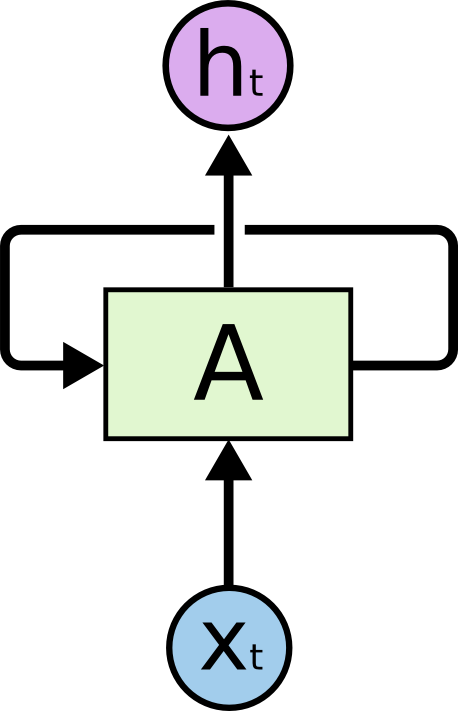
\includegraphics[width=2cm]
    {figure/model/RNN-rolled.png}}
    \caption{\label{fig:rnn-rolled} Recurrent Neural Network có vòng lặp.}
\end{figure}

Trong sơ đồ trên, một đoạn của mạng thần kinh, \(A\), xem xét một số xt đầu vào và xuất ra một giá trị
\(h_t\).Một vòng lặp cho phép thông tin được truyền từ một bước của mạng sang bước tiếp theo.

Những vòng lặp này làm cho Recurrent neural network có vẻ như bí ẩn.
Tuy nhiên, nếu bạn suy nghĩ nhiều hơn một chút, hóa ra họ không phải là một mạng lưới thần kinh bình thường.
Recurrent neural network có thể được coi là nhiều bản sao của cùng một mạng, mỗi bản tin truyền cho một người kế nhiệm.
Xem xét những gì xảy ra nếu chúng ta bỏ vòng lặp:

\begin{figure}[!htb]
    \center{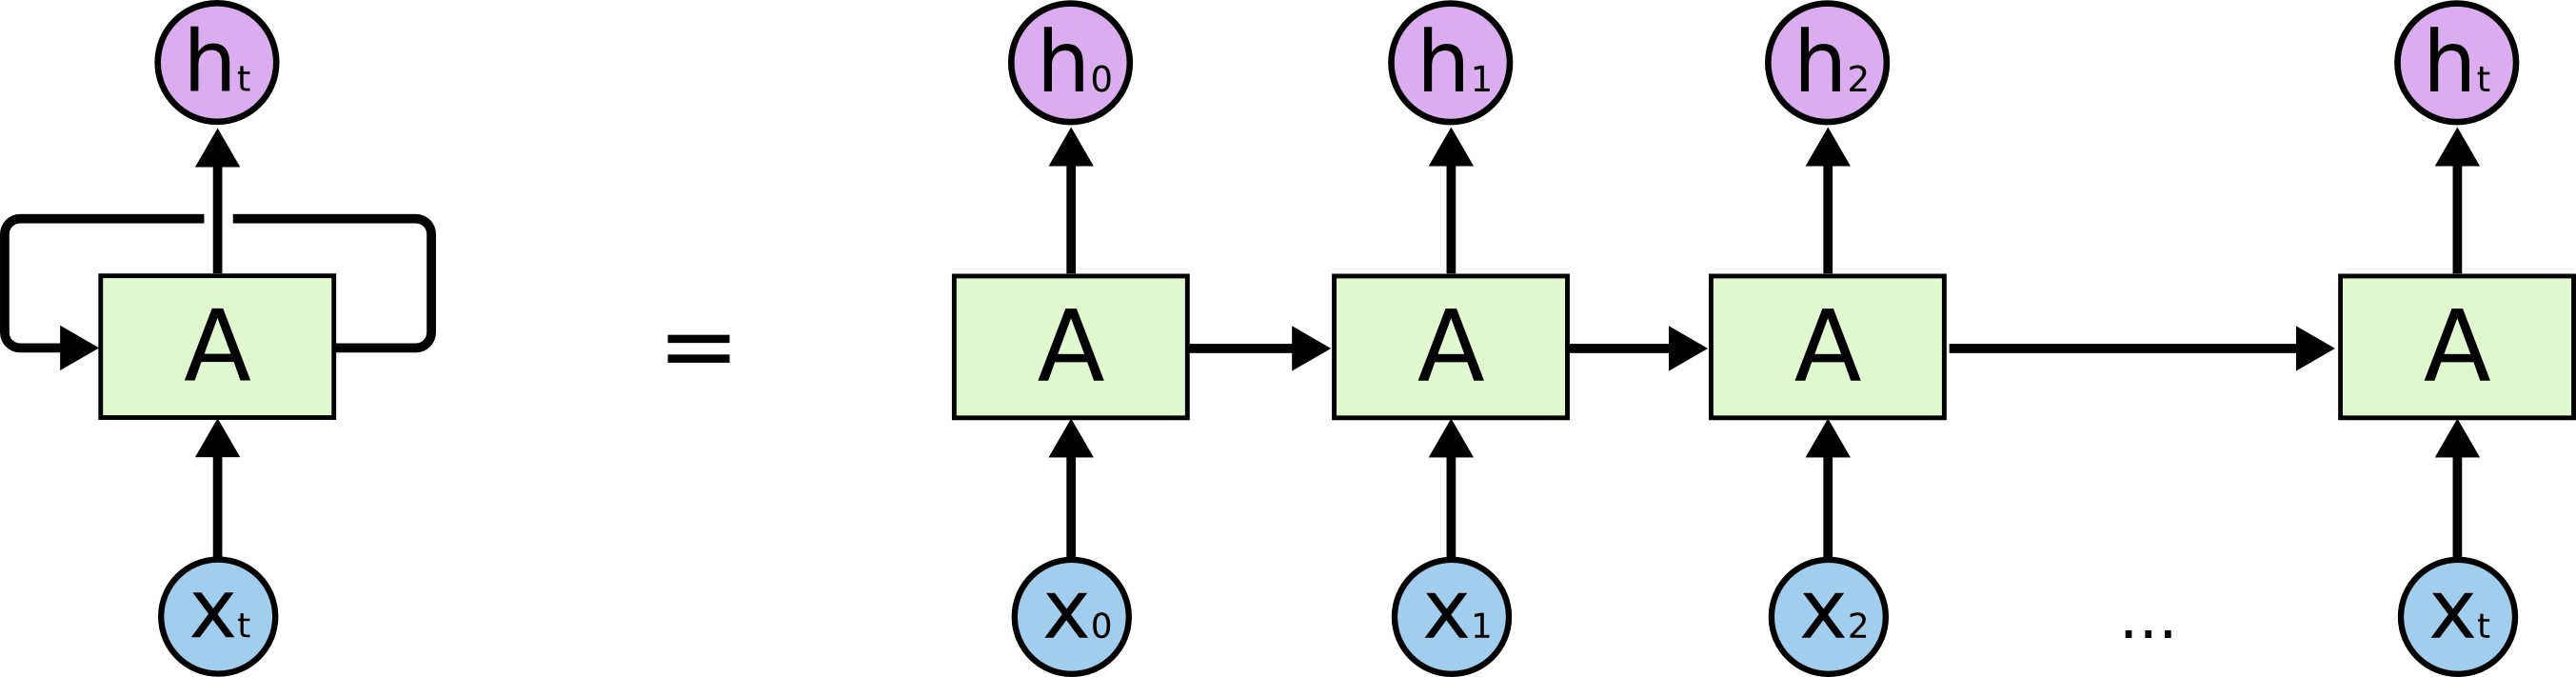
\includegraphics[width=\figureBigSize]
    {figure/model/RNN-unrolled.png}}
    \caption{\label{fig:rnn-unrolled} Recurrent Neural Network đã được trải ra.}
\end{figure}

Bản chất giống như chuỗi này cho thấy các Recurrent neural network có liên quan mật thiết đến các chuỗi và danh sách.
Nó sử dụng kiến trúc tự nhiên của mạng neuron để sử dụng cho dữ liệu đó.

Và chúng chắc chắn được sử dụng!
Trong vài năm qua, đã có những thành công đáng kinh ngạc khi áp dụng RNN cho nhiều vấn đề khác nhau: nhận dạng giọng
nói, mô hình ngôn ngữ, dịch thuật, chú thích hình ảnh.

Điều cần thiết cho những thành công này là việc sử dụng "LSTM", một loại Recurrent neural network rất đặc biệt, hoạt
động, cho nhiều tác vụ, tốt hơn nhiều so với phiên bản tiêu chuẩn. Hầu như tất cả các kết quả thú vị dựa trên các mạng thần kinh tái phát đều đạt được với chúng. Nó có những LSTM mà bài tiểu luận này sẽ khám phá.

\textbf{Vấn đề phụ thuộc xa} \\[0.2em]
Một trong những lời kêu gọi của RNN là ý tưởng rằng họ có thể kết nối thông tin trước đó với tác vụ hiện tại, chẳng
hạn như sử dụng các khung video trước đó có thể thông báo cho sự hiểu biết về khung hiện tại. Nếu RNN có thể làm điều
này, thì họ cực kỳ hữu ích. Nhưng họ có thể? Không hẳn.

Đôi khi, chúng ta chỉ cần nhìn vào thông tin gần đây để thực hiện nhiệm vụ hiện tại. Ví dụ, hãy xem xét một mô hình
ngôn ngữ đang cố gắng dự đoán từ tiếp theo dựa trên các từ trước đó. Nếu chúng ta đang cố gắng dự đoán từ cuối cùng
trong "các đám mây trên \textit{bầu trời}", thì chúng ta không cần bất kỳ bối cảnh nào nữa - đó là một điều khá rõ ràng,
từ tiếp theo sẽ là  \textit{bầu trời}. Trong những trường hợp như vậy, khi khoảng cách giữa thông tin liên quan và
địa điểm mà nó cần là nhỏ, RNN có thể học cách sử dụng thông tin trong quá khứ.

\begin{figure}[!htb]
    \center{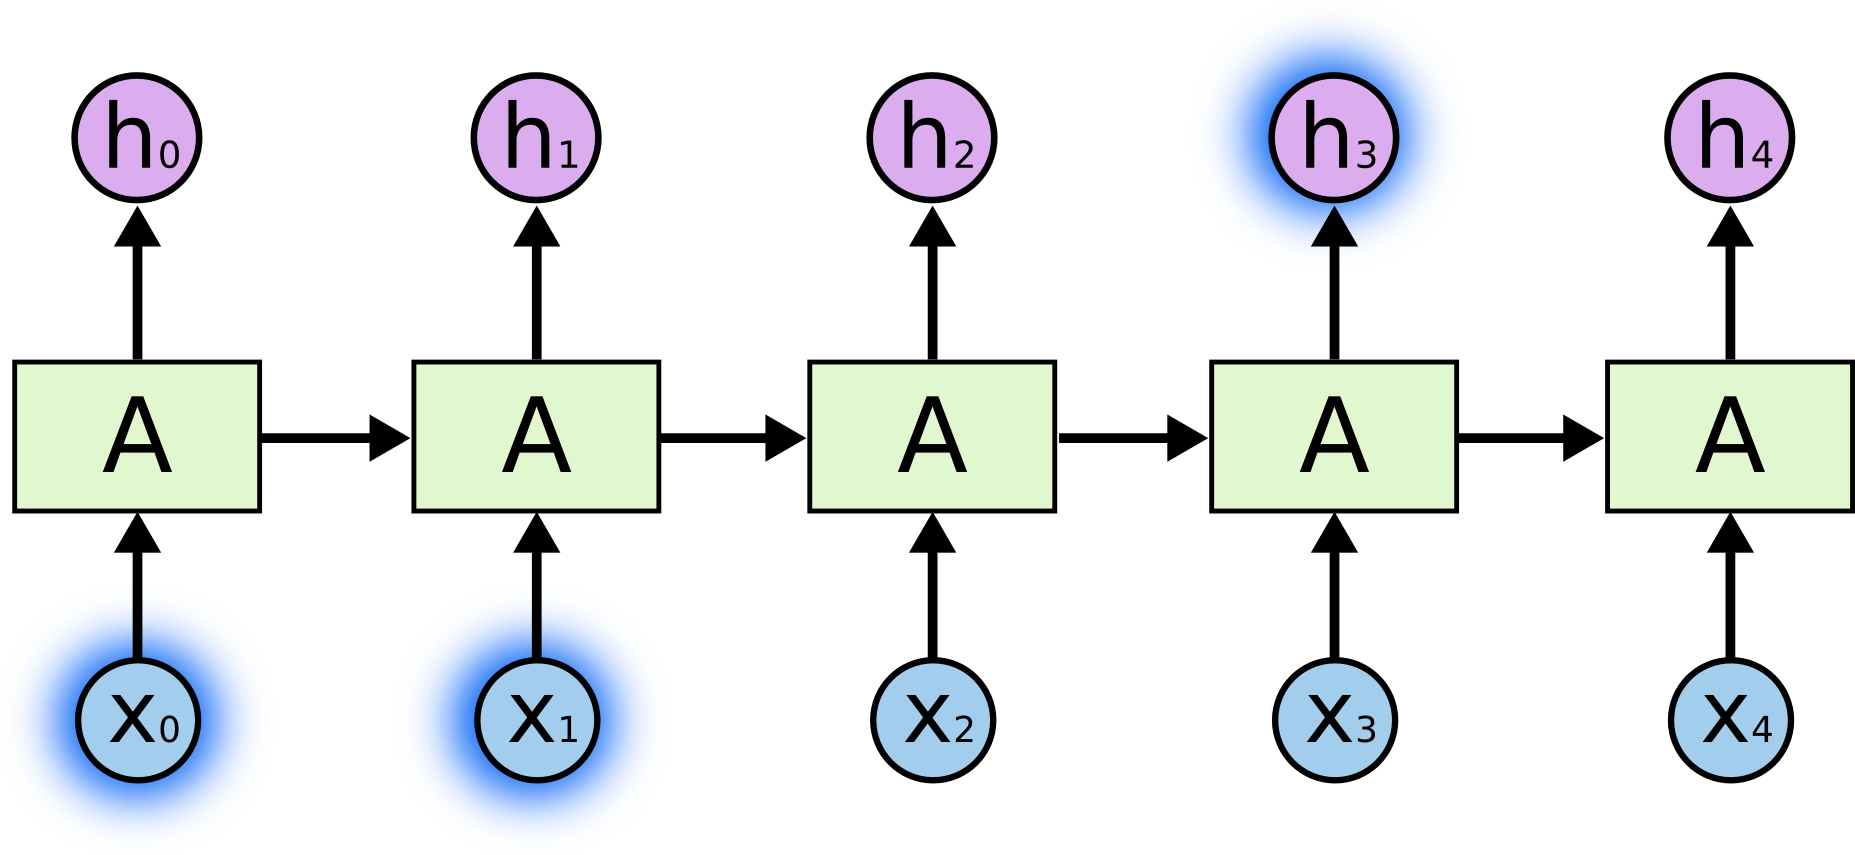
\includegraphics[width=\figureBigSize]
    {figure/model/RNN-shorttermdepdencies.png}}
\end{figure}

Nhưng cũng có những trường hợp chúng ta cần nhiều bối cảnh hơn. Cân nhắc việc cố gắng dự đoán từ cuối cùng trong văn
bản. "Tôi lớn lên ở Việt Nam. Tôi nói tiếng trôi chảy tiếng \textit{Việt}". Thông tin gần đây cho thấy từ tiếp theo có
lẽ là tên của một ngôn ngữ, nhưng nếu chúng ta muốn thu hẹp ngôn ngữ nào, chúng ta cần thu hẹp ngôn ngữ nào bối cảnh
của Việt Nam, từ phía trước. Nó hoàn toàn có thể cho khoảng cách giữa thông tin liên quan và điểm cần thiết để trở
nên rất lớn.

Thật không may, khi khoảng cách đó tăng lên, các RNN trở nên không thể học cách kết nối thông tin.
\begin{figure}[!htb]
    \center{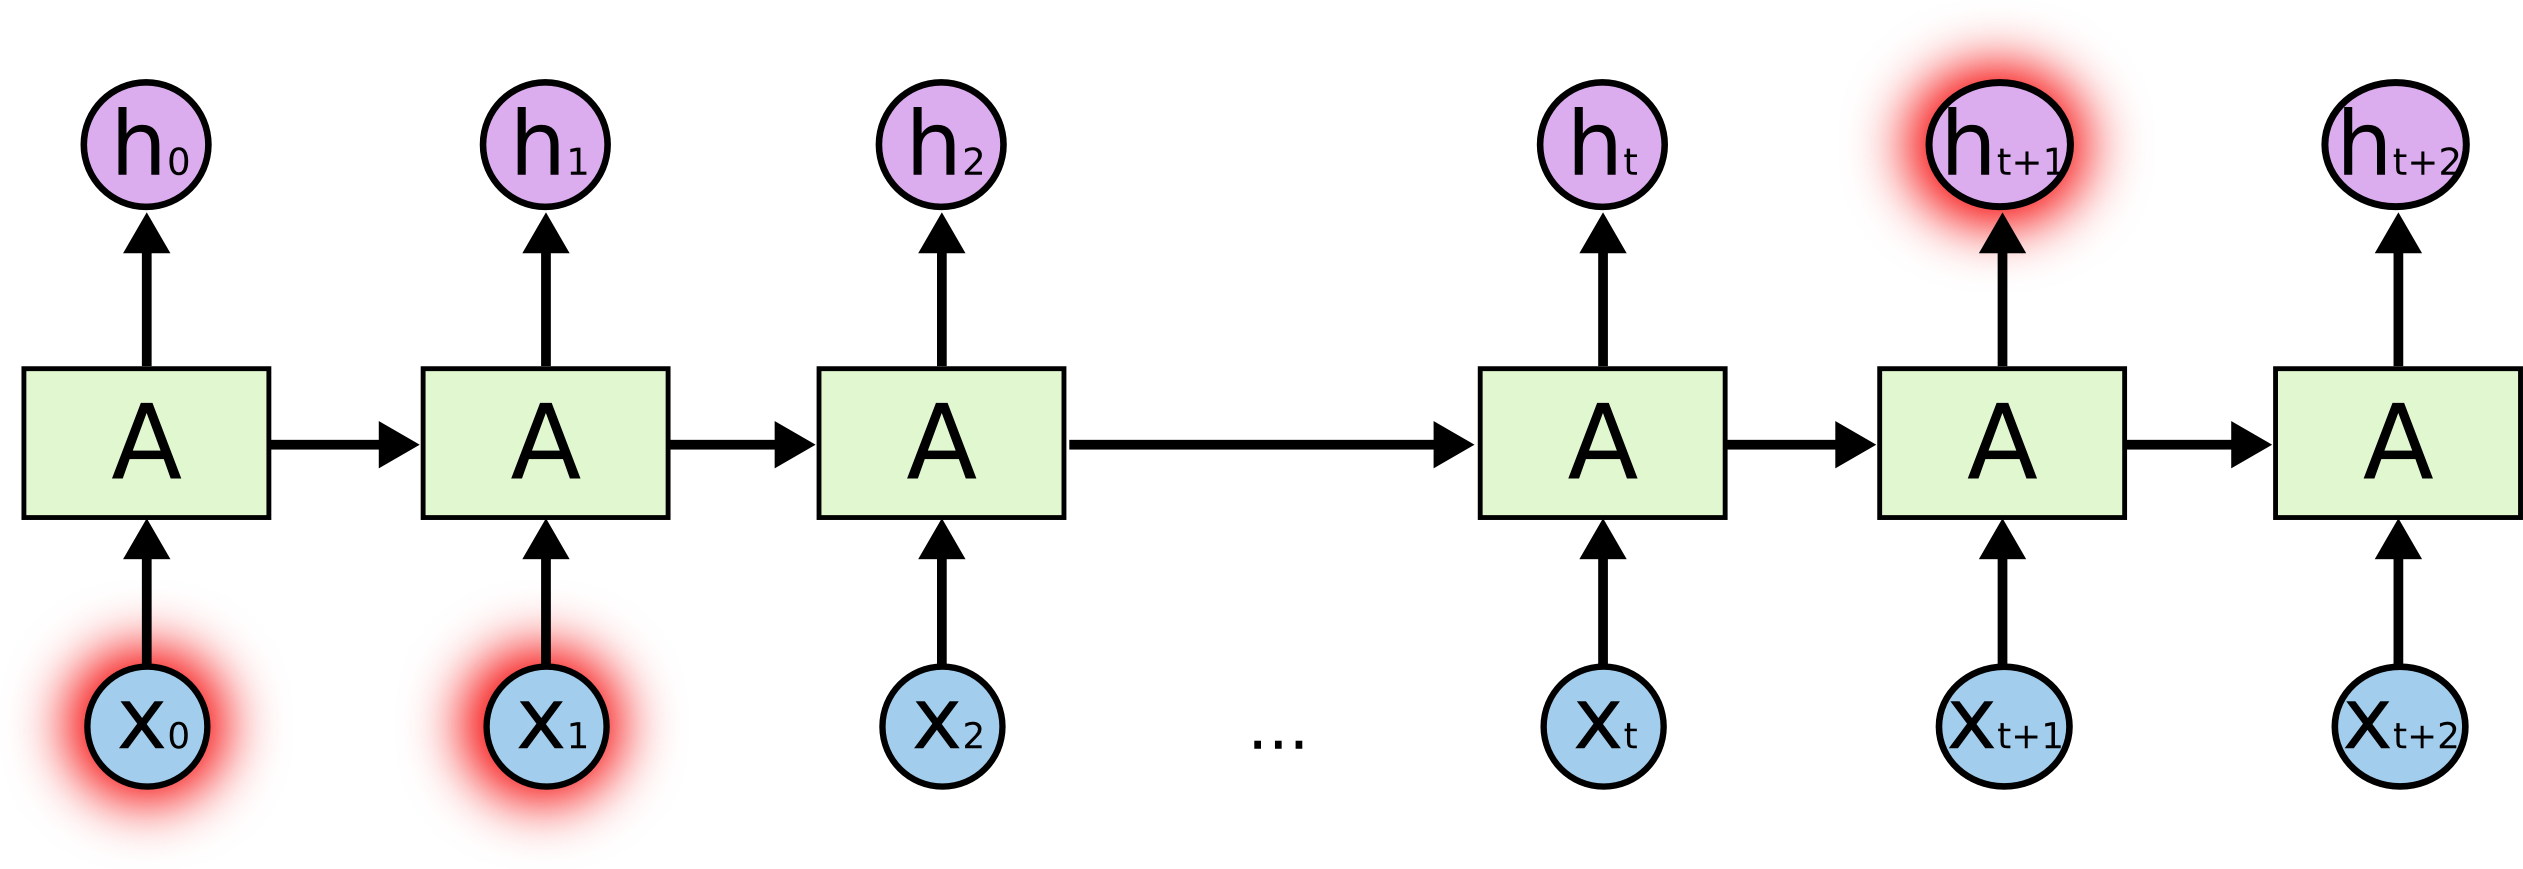
\includegraphics[width=\figureBigSize]
    {figure/model/RNN-longtermdependencies.png}}
\end{figure}


Về lý thuyết, các RNN hoàn toàn có khả năng xử lý các phụ thuộc dài hạn như vậy. Một người có thể cẩn thận chọn các
tham số cho họ để giải quyết các vấn đề về đồ chơi theo hình thức này. Đáng buồn thay, trong thực tế, RNNs don lồng
dường như có thể học chúng. Vấn đề đã được khám phá sâu bởi Hochreiter (1991) [German] và Bengio, et al. (1994),
người đã tìm thấy một số lý do khá cơ bản tại sao nó có thể khó khăn.

Rất may, LSTMs không có vấn đề này!

\textbf{Mạng LSTM} \\[0.2em]

Long Short Term Memory (mạng bộ nhớ dài ngắn hạn) - thường được gọi là LSTM của - - là một loại RNN đặc biệt, có khả
năng học các phụ thuộc xa. Chúng được giới thiệu bởi Hochreiter & Schmidhuber (1997), và được nhiều người tinh
chỉnh và phổ biến. Chúng hoạt động rất tốt trong nhiều vấn đề lớn, và hiện đang được sử dụng rộng rãi.

Các LSTM được thiết kế rõ ràng để tránh vấn đề phụ thuộc dài hạn. Ghi nhớ thông tin trong thời gian dài thực tế là
hành vi mặc định của nó, không phải là thứ khó khăn để học!

Tất cả các mạng thần kinh tái phát có dạng một chuỗi các module lặp lại của mạng thần kinh. Trong các RNN tiêu chuẩn,
module lặp lại này sẽ có cấu trúc rất đơn giản, chẳng hạn như một lớp \(tanh\) duy nhất.

\begin{figure}[!htb]
    \center{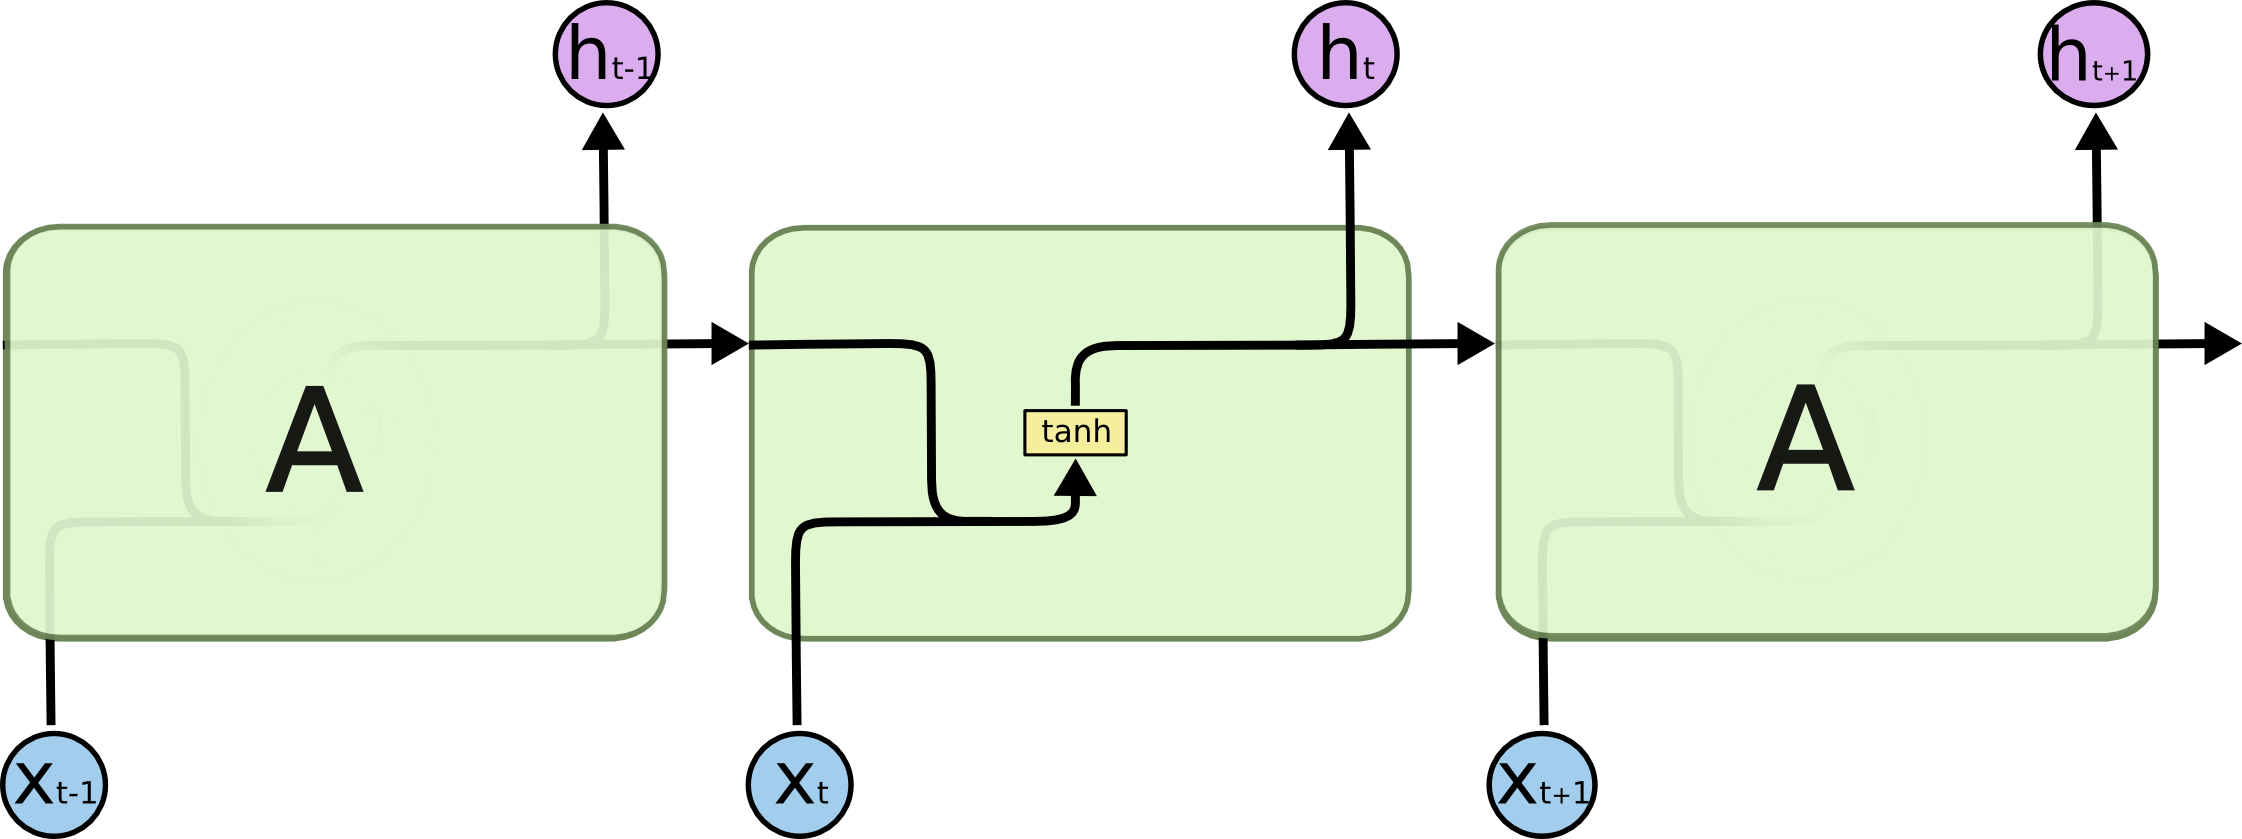
\includegraphics[width=\figureBigSize]
    {figure/model/LSTM3-SimpleRNN.png}}
    \caption{\label{fig:lstm3-simpleRNN} Module lặp trong RNN chuẩn chứa một lớp duy nhất.}
\end{figure}

LSTMs cũng có cấu trúc chuỗi, nhưng các module lặp có một cấu trúc khác. Thay vì có một lớp
mạng thần kinh duy nhất,nó có bốn lớp, tương tác theo một cách rất đặc biệt.

\begin{figure}[!htb]
    \center{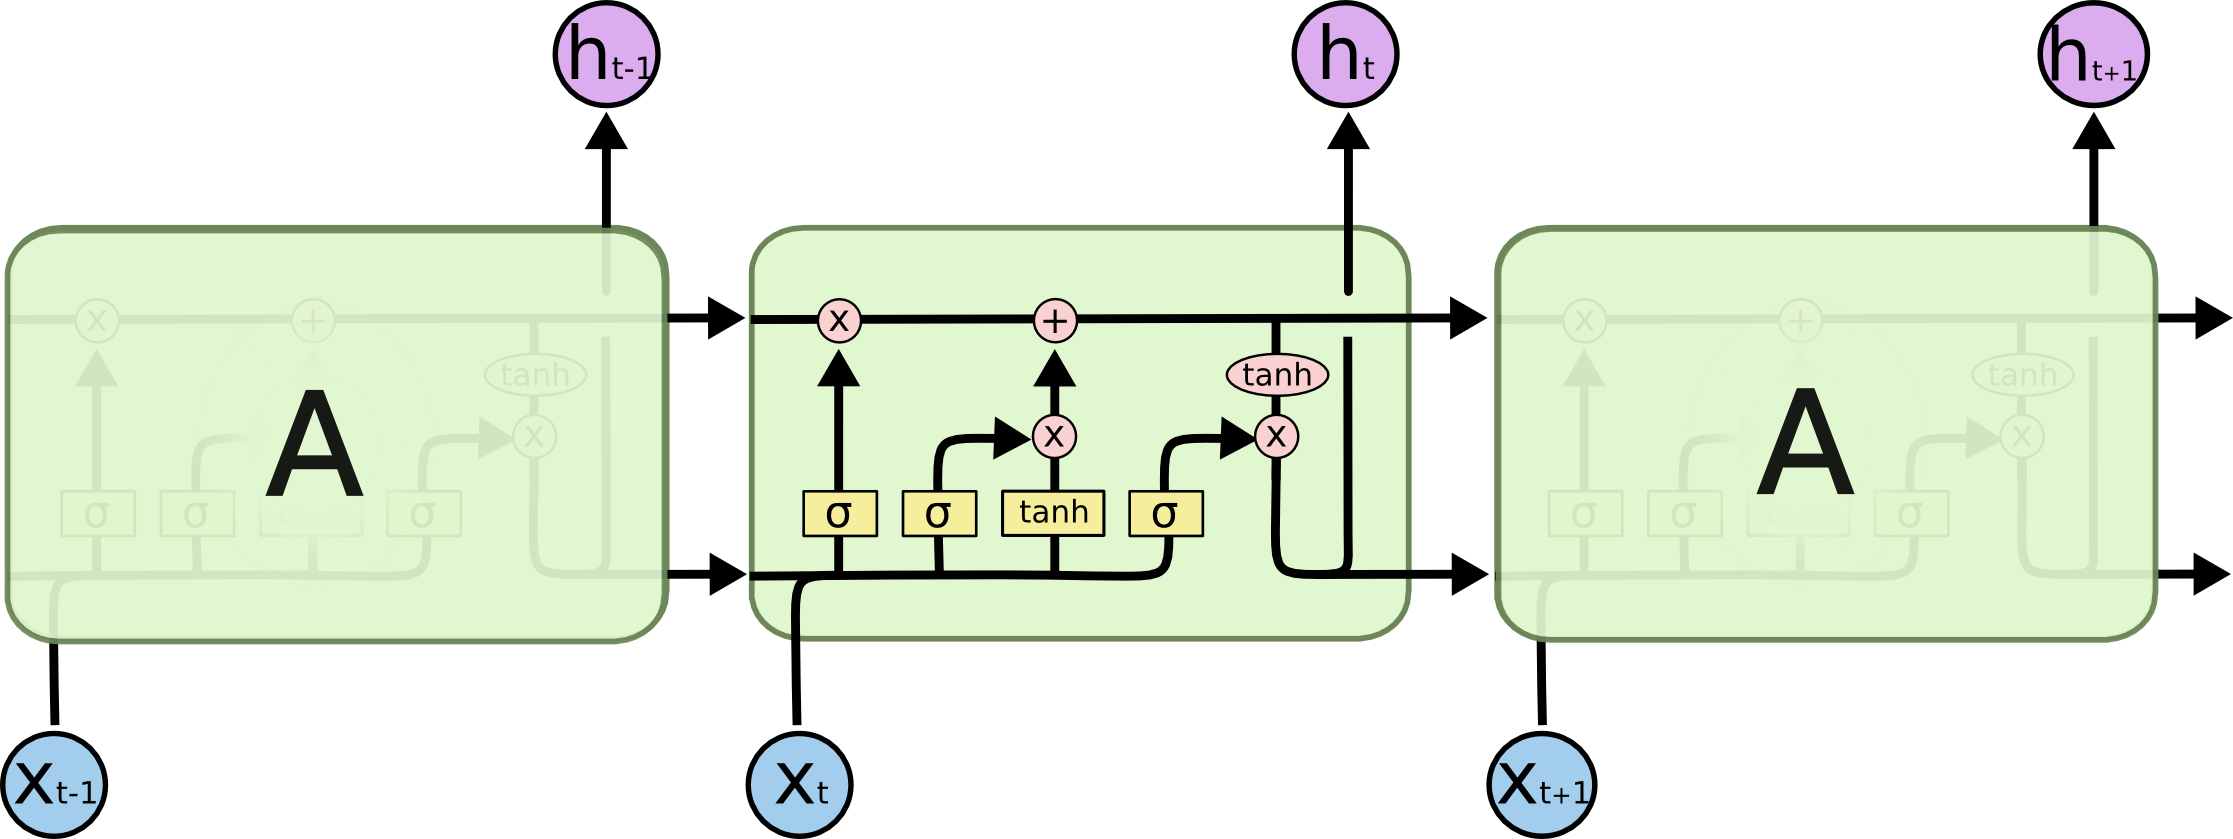
\includegraphics[width=\figureBigSize]
    {figure/model/LSTM3-chain.png}}
    \caption{\label{fig:lstm3-chain} Module lặp trong LSTM chứa 4 lớp tương tác.}
\end{figure}

\begin{figure}[!htb]
    \center{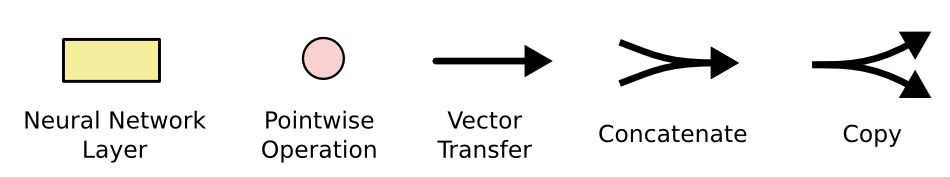
\includegraphics[width=\figureBigSize]
    {figure/model/LSTM2-notation.png}}
    \caption{\label{fig:lstm2-notation} Các ký hiệu trong LSTM.}
\end{figure}

Trong sơ đồ trên, mỗi dòng mang toàn bộ một vector, từ đầu ra của một nút đến đầu vào của các nút khác. Các vòng tròn
màu hồng đại diện cho các phép toán, như phép cộng vector, trong khi các hình chữ nhật màu vàng biểu thị các mạng
thần kinh để học. Các dòng hợp nhất biểu thị việc ghép nối, trong khi một dòng phân tách biểu thị nội dung của nó được
sao chép và các bản sao đi đến các vị trí khác nhau.

\textbf{Ý tưởng chính của LSTM} \\[0.2em]

Ý tưởng chính của LSTM là ô trạng thái, đường ngang chạy qua đỉnh sơ đồ.

Dòng trạng thái giống như một băng chuyền. Nó chạy thẳng xuống toàn bộ chuỗi, chỉ với một số tương tác tuyến tính nhỏ
dọc bên cạnh, dễ dàng cho thông tin truyền theo.

\begin{figure}[!htb]
    \center{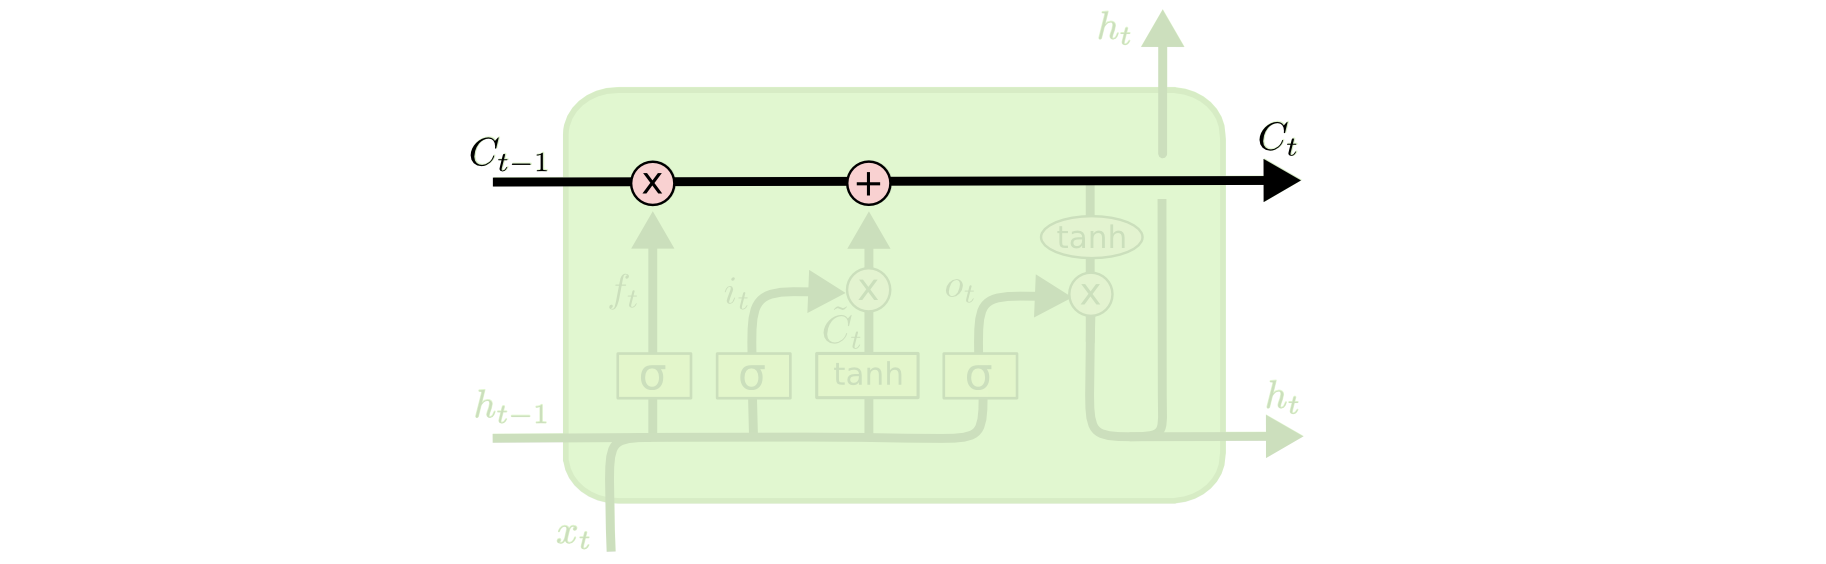
\includegraphics[width=\figureBigSize]
    {figure/model/LSTM3-C-line.png}}
\end{figure}

LSTM có khả năng loại bỏ hoặc thêm thông tin vào ô trạng thái, được điều chỉnh cẩn thận bởi các cấu trúc gọi là
cổng.

Cổng là một cấu trúc điều khiển thông tin thông qua. Chúng được cấu tạo từ một lớp lưới thần kinh \(sigmold\) và
một phép toán nhân.

\begin{figure}[!htb]
    \center{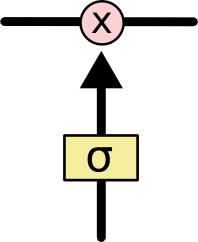
\includegraphics[width=1cm]
    {figure/model/LSTM3-gate.png}}
\end{figure}

Đầu ra của các lớp \(sigmoid\) có giá trị \([0, 1]\), mô tả mức độ cho qua. Giá
trị bằng \(0\) có nghĩa là không để bất cứ thứ gì qua, trong khi giá trị của \(1\) nghĩa
là có thể cho phép mọi thứ thông qua!

Một LSTM có ba trong cổng này, để bảo vệ và kiểm soát trạng thái tế bào.

\textbf{Các bước LSTM hoạt động} \\[0.2em]

Bước đầu tiên trong LSTM  là quyết định thông tin nào đi ra khỏi ô trạng thái. Quyết định này được đưa ra bởi
một lớp sigmoid được gọi là lớp "cổng quên". Nó dựa vào giá trị của \(h_{t-1}\) và \(x_t\), và đưa ra một số từ 0
đến 1 tương ứng với mỗi số ô trạng thái \(c_{t-1}\). Số 1 có nghĩa là giữ lại toàn bộ thông tin trong khi đó số 0 nghĩa
là hãy quên nó đi.

Hãy xem ví dụ của chúng ta về một mô hình ngôn ngữ đang cố gắng dự đoán từ tiếp theo dựa trên tất cả các từ trước đó.
Trong một vấn đề như vậy, ô trạng thái có thể bao gồm vai vế của ngữ hiện tại, để có thể sử dụng các đại từ nhân xưng
một cách chính xác. Khi có một chủ ngữ mới, nó sẽ quên đi vai vế của chủ ngữ cũ.

\begin{figure}[!htb]
    \center{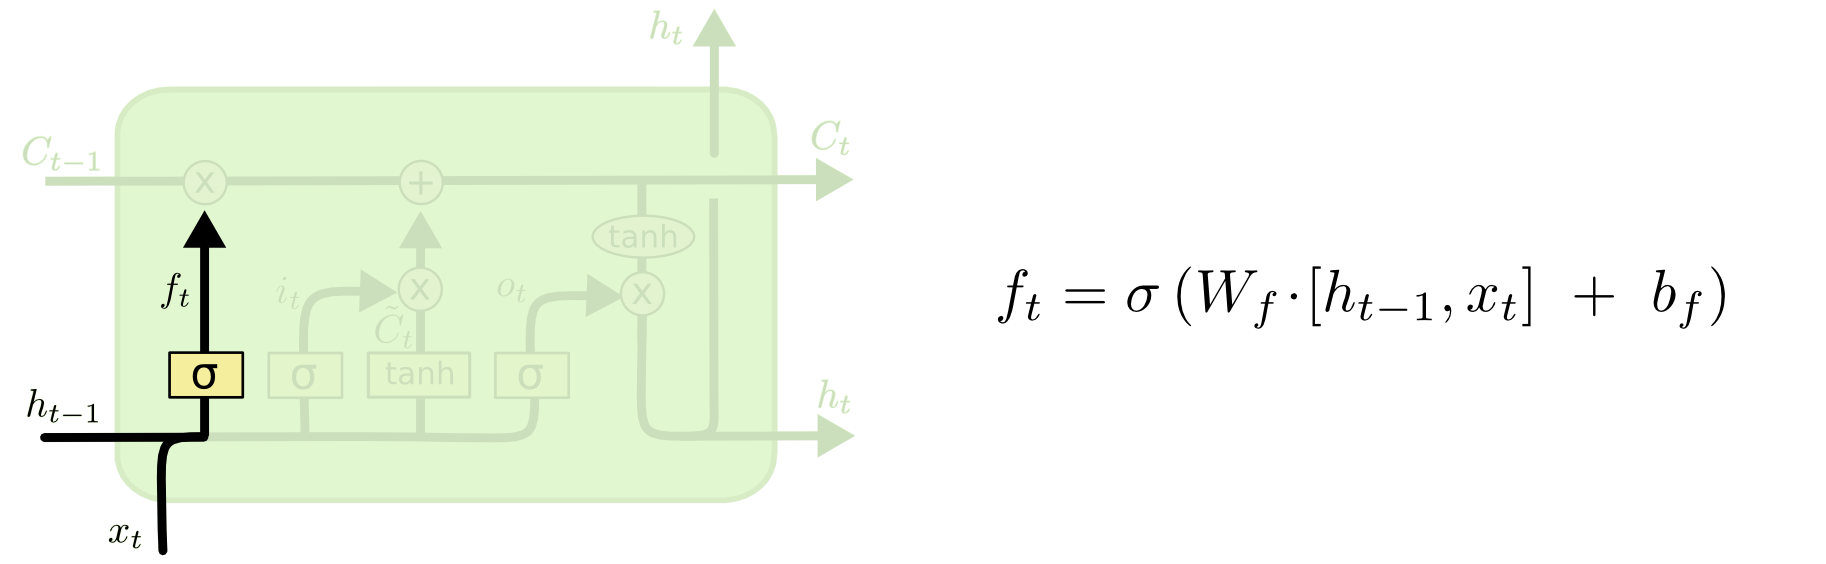
\includegraphics[width=\figureBigSize]
    {figure/model/LSTM3-focus-f.png}}
\end{figure}

Bước tiếp theo là quyết định những thông tin mới sẽ lưu trữ trong ô trạng thái. Việc này có hai phần. Đầu tiên,
một lớp sigmoid được gọi là lớp "cổng đầu vào" quyết định giá trị nào sẽ cập nhật. Tiếp theo, một lớp \(tanh\)
tạo ra một vector các giá trị ứng cử viên mới, \(C_t\), có thể được thêm vào ô trạng thái. Sau đó sẽ kết hợp  cả hai
để tạo ra một bản cập nhật cho trạng thái.

Trong ví dụ về mô hình ngôn ngữ, chúng tôi muốn thêm vai vế của chủ ngữ mới vào ô trạng thái, để thay thế chủ ngữ đã
quên.
\begin{figure}[!htb]
    \center{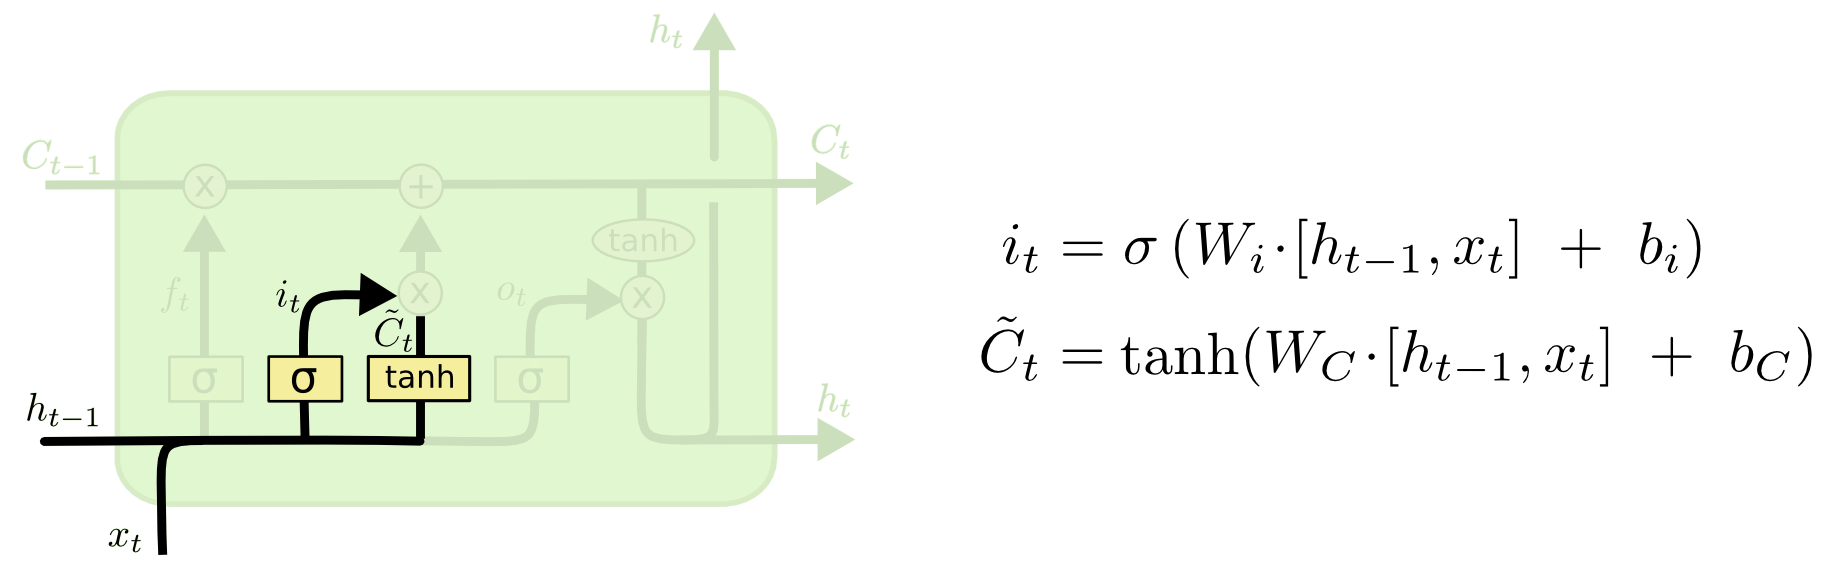
\includegraphics[width=\figureBigSize]
    {figure/model/LSTM3-focus-i.png}}
\end{figure}

Bây giờ, sẽ cập nhật ô trạng thái cũ, \(C_{t-1}\), sang ô trạng thái mới \(C_{t}\). Các bước trước đã quyết định phải
quên và nhớ những gì, giờ là lúc thực hiện nó.

Nhân ô trạng thái vũ với \(f_t\), quên đi những điều quyết định quên trước đó. Sau đó, cộng với \
i_t*\widetilde{C}_t\).
Đây là giá trị ứng viên mới, được tính theo mức độ cập nhật từng giá trị trạng thái.

Trong trường hợp của mô hình ngôn ngữ, đây là lúc thực sự bỏ thông tin về vai về và thêm thông tin mới, như đã quyết định trong các bước trước.
\begin{figure}[!htb]
    \center{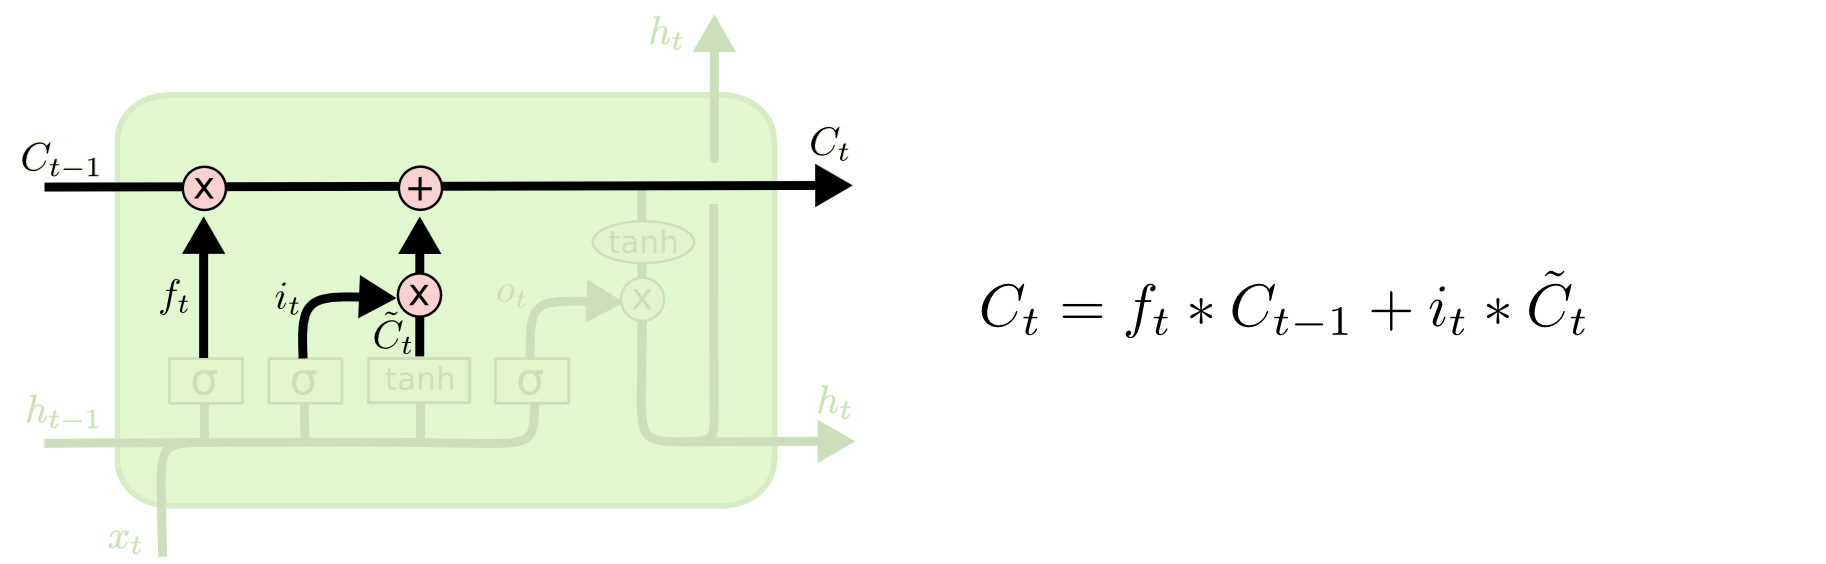
\includegraphics[width=\figureBigSize]
    {figure/model/LSTM3-focus-C.png}}
\end{figure}
Cuối cùng là quyết định những gì sẽ xuất ra. Đầu ra sẽ được lọc dựa vào ô trạng thái. Đầu tiên, chạy một lớp
\(sigmoid\) quyết định phần nào của ô trạng thái mà sẽ xuất ra. Sau đó, đưa ô trạng thái qua hàm
\(tanh\) (để đẩy các giá trị nằm trong khoảng -1 đến 1) và nhân nó với đầu ra của cổng \(sigmoid\), do đó chỉ đưa ra
các dữ liệu đã quyết định

Đối với ví dụ về mô hình ngôn ngữ, vì nó chỉ nhìn thấy một chủ ngữ, nó có thể muốn đưa ra thông tin có liên quan đến
một động từ, trong trường hợp đó là những gì sắp diễn ra. Ví dụ, nó có thể xuất ra vai vế của chủ ngữ , để biết được
cách dùng từ với chủ ngữ đó.